

\documentclass[12pt,a4paper]{article}
\newcommand\persiangloss[2]{#1\dotfill\lr{#2}\\}
\usepackage{graphicx}
\usepackage{xcolor}
\usepackage{listings}
\usepackage{indentfirst}
\usepackage{float}
\usepackage[pagebackref=false,colorlinks,linkcolor=blue,citecolor=magenta]{hyperref}
\usepackage{xepersian}
\settextfont{XB Niloofar}
\definecolor{vgreen}{RGB}{104,180,104}
\definecolor{vblue}{RGB}{49,49,255}
\definecolor{vorange}{RGB}{255,143,102}

\lstdefinestyle{verilog-style}
{
	language=C,
	basicstyle=\small\ttfamily,
	keywordstyle=\color{vblue},
	identifierstyle=\color{black},
	commentstyle=\color{vgreen},
	numbers=left,
	numberstyle=\tiny\color{black},
	numbersep=10pt,
	tabsize=8,
	moredelim=*[s][\colorIndex]{[}{]},
	literate=*{:}{:}1
} 



\begin{document}
	\thispagestyle{empty}
	\vspace*{0mm}
	\centerline{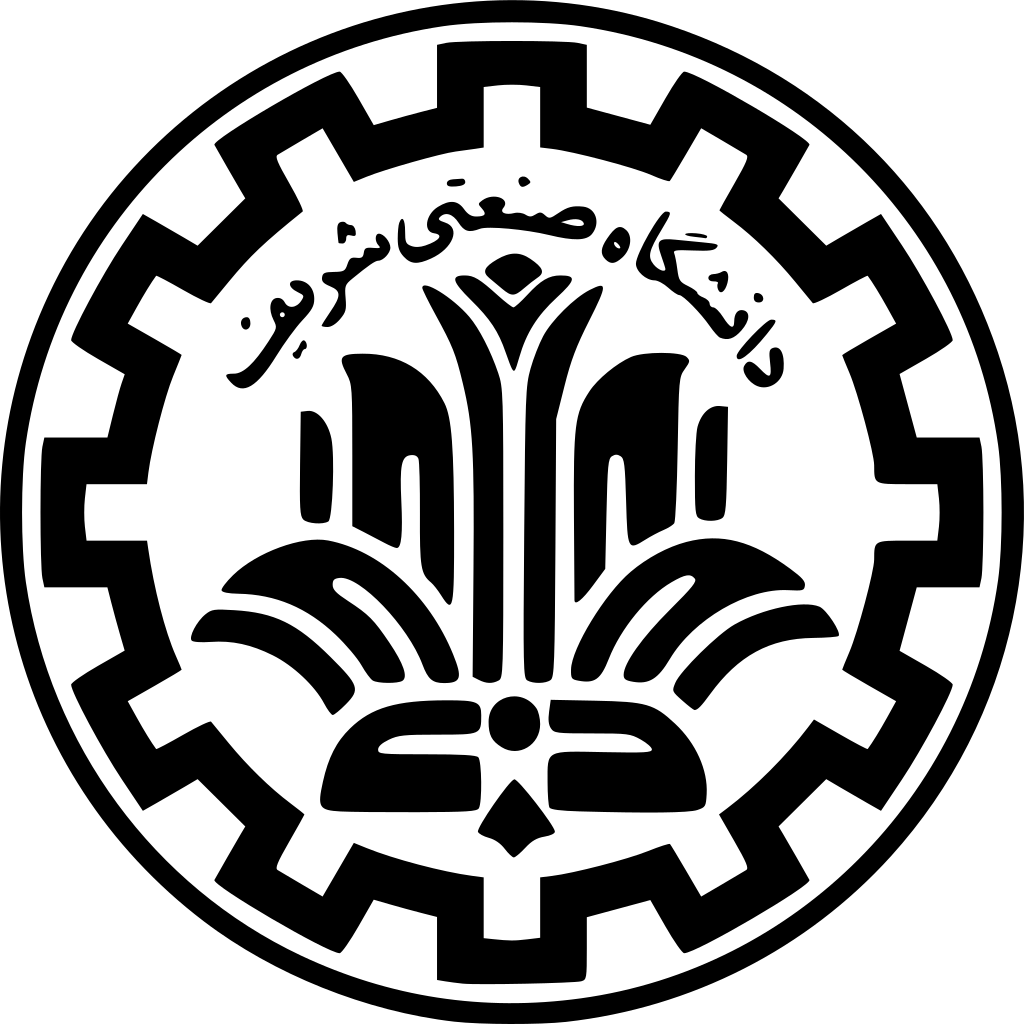
\includegraphics[height=4cm]{logo.png}}
	\vspace*{5mm}
	\begin{center}
		{\Huge
			لوستر هوشمند
		}
		\\[1cm]
		آزمایشگاه سخت‌افزار
		\\[1cm]
		دانشکده مهندسی کامپیوتر
		\\[4cm]
		{\large
			محمدرضا عبدی ۹۷۱۱۰۲۸۵
			
			حمیدرضا کامکاری ۹۷۱۱۰۱۷۷
			
			یگانه قره‌داغی 97106216
		}
		\\[5cm]
		خرداد ۱۴۰۱
	\end{center}
	\newpage
	
	\section*{مقدمه}
	
	روند خودکار سازی فعلی خانه‌ها قدمی مهم برای کاهش مصرف بی‌اندازه برق و تسهیل زندگی افراد خانه است. انواع لوستر‌ها و تجهیزات روشنایی از جدیدترین وسایل اضافه شده به لوازم خانگی هوشمند هستند. هدف از این پروژه طراحی یک لوستر هوشمند است که بتواند به کمک یک برنامه به لوازم جانبی هوشمند دیگر (مانند تلفن‌های همراه) متصل شود و توسط آن به صورت خودکار یا دستی تنظیم شود. این دستگاه جزو یک شبکه اینترنت اشیا (\lr{Internet of Things}) است و با استفاده از یک برنامه موبایل قابل مدیریت است. 
	
	در این گزارش به توضیح قابلیت‌ها، محدودیت‌ها، قطعات و جزئیات پیاده‌سازی لوستر هوشمند در ۶ بخش می‌پردازیم.
	
	\section{قابلیت‌های لوستر هوشمند}
	با توجه به اهداف پروژه در خودکار سازی روشنایی خانه\footnote{کاهش مصرف برق و تسهیل استفاده نسبت به لوسترهای مرسوم}، قابلیت‌های زیر برای محصول در نظر گرفته شده‌اند\footnote{جزئیات قابلیت‌ها در توصیف برنامه موبایل به صورت کامل توضیح داده‌ می‌شود}:
	
	\begin{itemize}
		\item
		در اولین مرحله این لوستر می‌تواند به کمک سنسوری بر اساس شرایط محیطی مانند وضعیت پرده‌ها یا روشنایی طبیعی بازخورد بدهد؛ در صورت زیاد بودن شدت نور محیط، روشنایی لوستر کاهش و در صورت کم بودن شدت نور افزایش می‌یابد. میزان حساسیت نسبت به روشنایی و میزان روشنایی مورد نیاز می‌تواند بر اساس نیاز کاربر تغییر کند. به عنوان مثال پارامتر‌ اندازه اتاق می‌تواند در تنظیمات تاثیر داده شود. یعنی برای اتاق‌های بزرگتر شدت نور به هنگام روشن بودن بیشتر باشد. 
		\item
		می‌توان تنظیمات روشنایی لوستر را به صورت خودکار یا دستی تنظیم کرد. در صورت انتخاب حالت دستی، کاربر می‌تواند میزان روشنایی ثابتی را انتخاب کند.
		\item
		کاربر می‌تواند شاخه (اتاق‌های مختلف خانه) دلخواه خود را انتخاب کند و تنظیمات هر کدام از قسمت‌ها را به صورت جداگانه انجام دهد.
		\item
		کاربر می‌تواند از میان حالت‌های‌ \footnote{Mode} مختلف ارائه شده برای زیبایی یا رقص نور استفاده نماید.
	\end{itemize}
	
	\section{محدودیت‌های اولیه پروژه}
	
	در هنگام پیاده‌سازی و استفاده از پروژه با محدودیت‌هایی مواجه می‌شویم که در ادامه آن‌ها را تشریح می‌کنیم:
	
	\begin{itemize}
		\item
		چالش اصلی اتصال تعداد زیادی دیود ساطع نور \lr{LED\footnote{\lr{Light-emitting diode}}} با نورهای متغیر به برد برای شبیه‌سازی یک لوستر واقعی است. در نهایت با اتصال ۴۰ قطعه \lr{LED} به یک منبع خارجی ۵ ولت و کنترل آن بویسله خروجی \lr{PWM} و دو ترانزیستور (برای دو شاخه) لوستر را شبیه‌سازی کردیم.
		\item
		در برخی موارد، برنامه‌های گوشی‌های هوشمند با اتصال خود به سیستم روشنایی سازگار نیستند. در این پروژه سعی شده‌است که یک برنامه موبایل سازگار با سیستم‌عامل‌های مانند \lr{Android}و \lr{IOS} مختلف برای برطرف شدن این مشکل ارائه شود.
		\item
		با وجود اینکه این موضوع کمتر و کمتر اتفاق می‌افتد، اما هر اتصال \lr{WiFi}‌ای گاهی اوقات دچار اختلال می‌شود. با توجه به اینکه لوستر هوشمند بستری بر پایه \lr{IoT} است، بدون اتصال \lr{WiFi} نمی‌توان از تنظیمات لوستر بهره برد. بنابراین پیشنهاد می‌شود که دکمه‌ها و یا کلید‌های سخت‌افزاری همچنان برای تنظیمات پایه‌ موجود باشد.
	\end{itemize}
	
	\section{قطعات مورد استفاده}
	لوستر از دو شاخه \lr{LED} تشکیل شده و میزان ولتاژ ورودی هر کدام از این شاخه‌ها از طریق پورت مربوطه روی بورد \lr{Arduino} و ترانزیستور (\lr{MOSFET IRF640}) کنترل می‌شود. برای پیاده‌سازی منطق لوستر از بورد \lr{Arduino Mega} استفاده می‌کنیم که از طریق سنسور‌های تشخیص نور (\lr{BH1750FVI}) نور محیط را تشخیص می‌دهد و بر اساس پیش‌فرض‌هاییکه در سرور \lr{IOT} چیده‌شده میزان ولتاژ خروجی‌های آنالوگ را تنظیم می‌کند. از طرفی برای اتصال به اینترنت اشیا یک سرور کوچک خانگی را روی ماژول \lr{ESP8266 ESP-01S} اجرا می‌کنیم. این سرور تنظیمات کنترل لوستر را در خود دارد و با استفاده از گوشی همراه و اتصال به آن سرور می‌توانیم این تنظیمات را کنترل کنیم.
	
	لیست قطعات و شرح پین‌های آن‌ها به شرح زیر است:
	\begin{enumerate}
		\item {
			سنسور روشنایی : \lr{BH1750FVI}
			\footnote{	ما مقادیر \lr{lux} را از \lr{BH1750} از طریق باس \lr{I2C} دریافت می کنیم. \lr{ADC} در \lr{IC} روشنایی آنالوگ را به مقدار لوکس دیجیتال تبدیل می‌کند. سپس این داده‌ها با کمک پین‌های \lr{I2C} یعنی \lr{SCL} و \lr{SDA} به میکروکنترلر منتقل می‌شوند. \lr{SCL} برای ارائه پالس ساعت و \lr{SDA} برای انتقال مقدار \lr{lux} استفاده می‌شود.}}
		
		\begin{figure}[H]
			\centering
			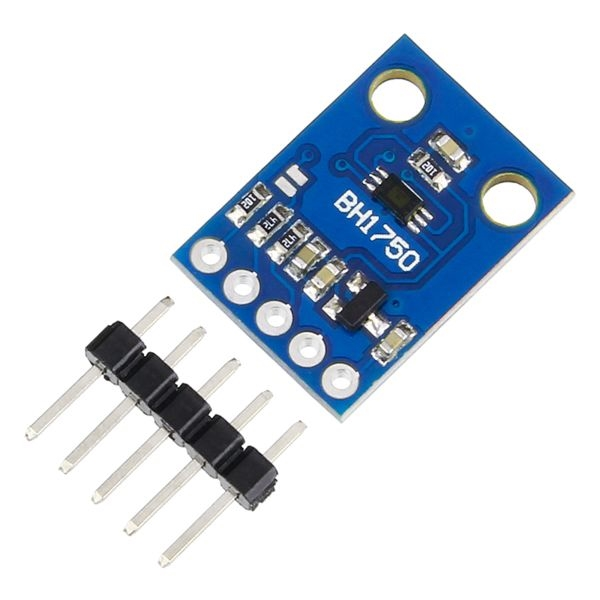
\includegraphics[scale=0.2]{figs/BH1750FVI.jpeg}
			\caption{
				سنسور روشنایی \lr{BH1750FVI}
			}
			\label{fig:schema}
		\end{figure}
		
		\begin{figure}[H]
			\centering
			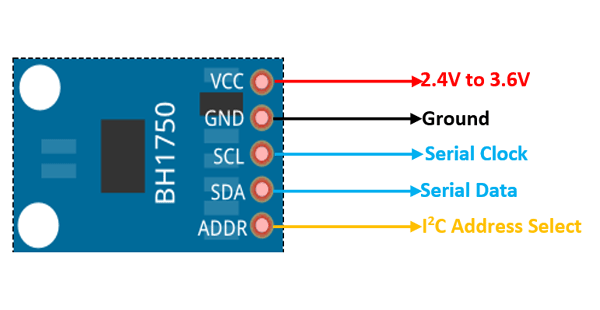
\includegraphics[scale=0.3]{figs/BH1750-Light-Sensor-Pinout.png}
			\caption{
				شرح پین‌های \lr{BH1750FVI}
			}
			\label{fig:schema}
		\end{figure}
		
		\begin{figure}[H]
			\centering
			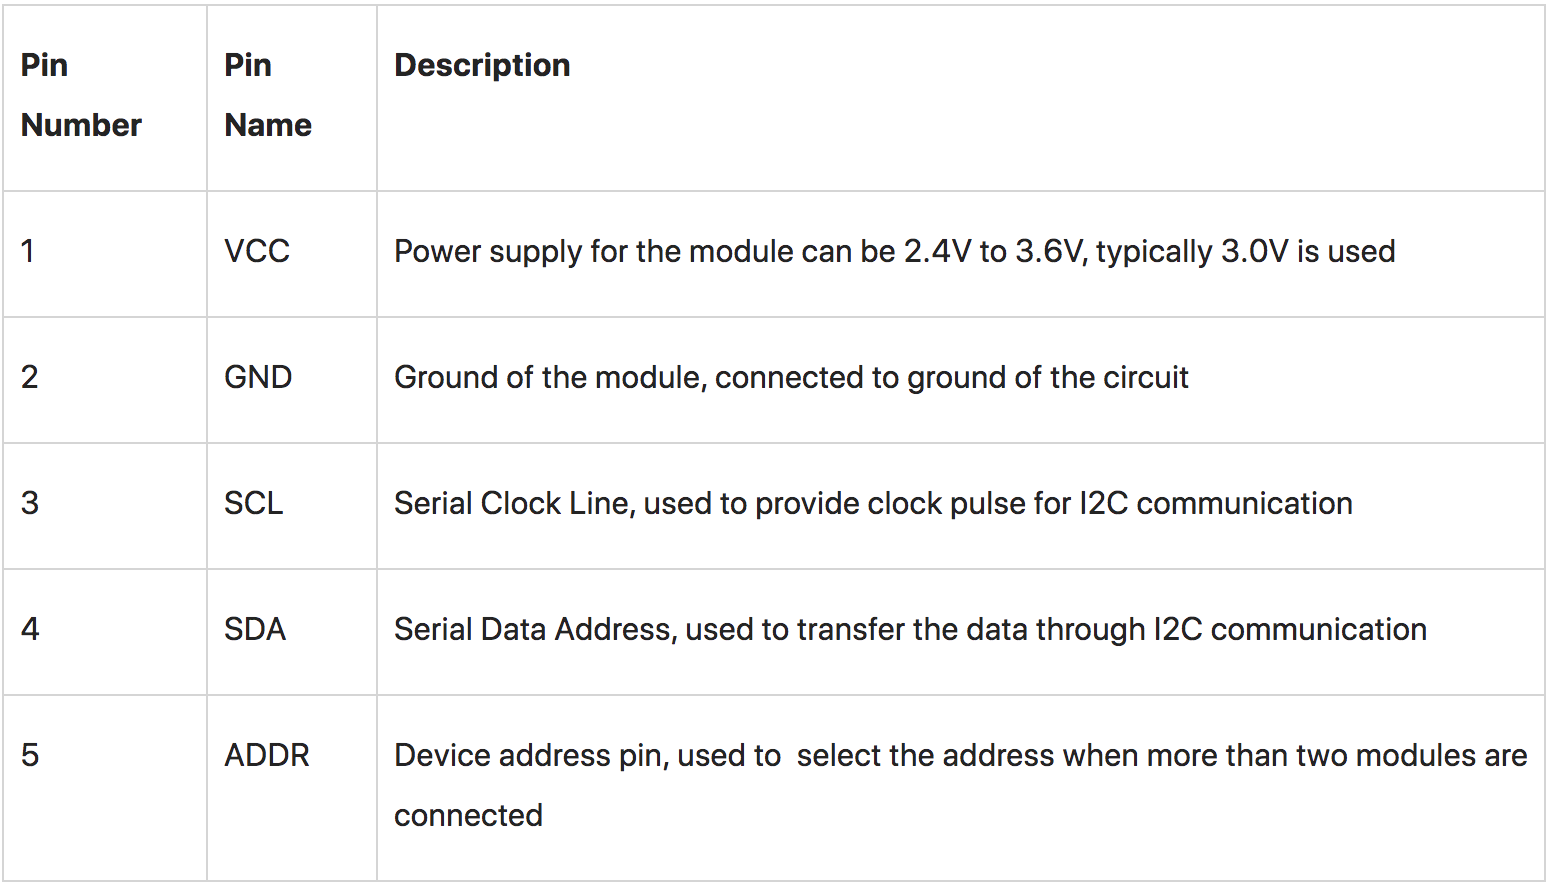
\includegraphics[scale=0.4]{figs/BH1750FVI-pin-config.png}
			\caption{
				تنظیمات پین‌های \lr{BH1750FVI}
			}
			\label{fig:schema}
		\end{figure}	
		
		\item {
			برد آردویینو مگا : \lr{Arduino Mega 2560 R3}
		}
		
		\begin{figure}[H]
			\centering
			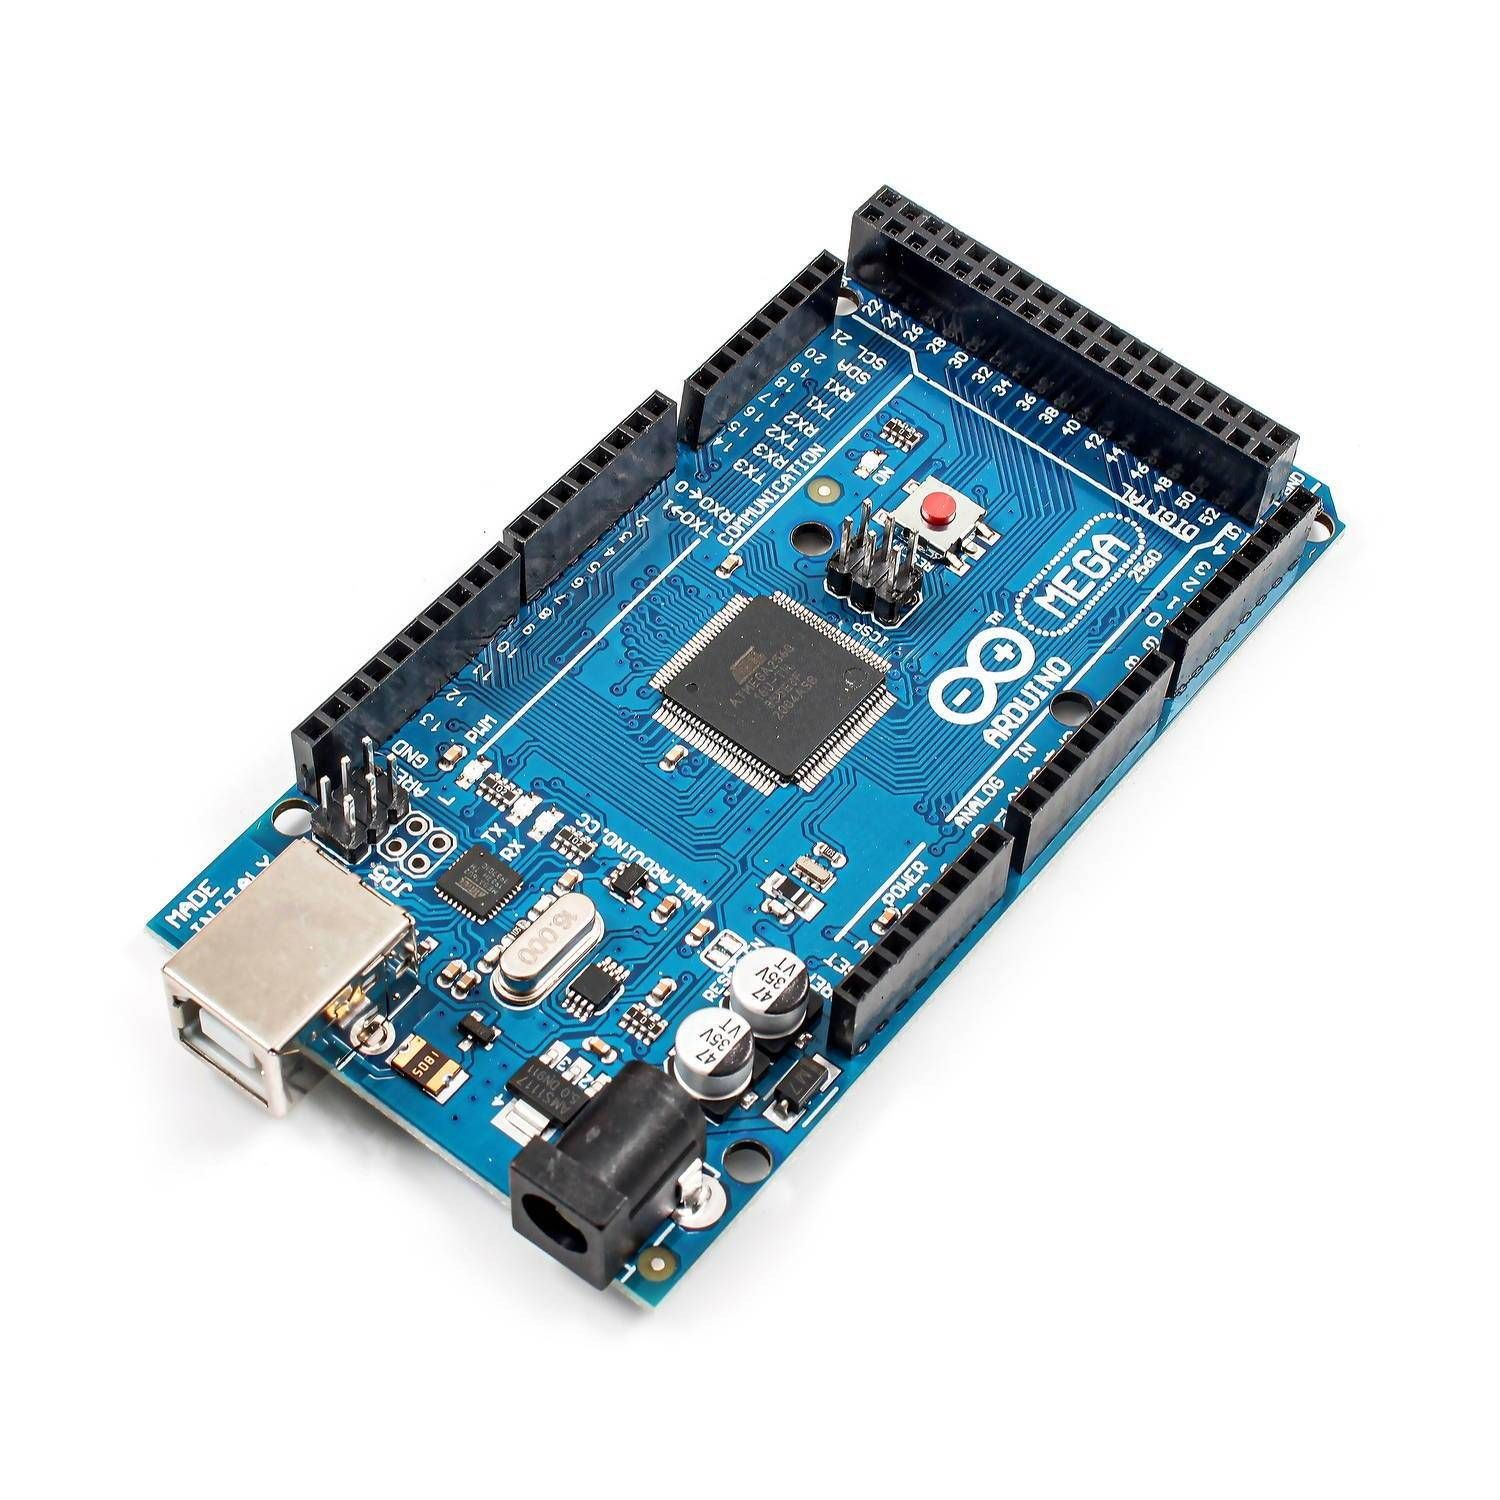
\includegraphics[scale=0.1]{figs/ard-mega.jpeg}
			\caption{
				برد \lr{Arduino Mega 2560 R3}
			}
			\label{fig:schema}
		\end{figure}
		
		\begin{figure}[H]
			\centering
			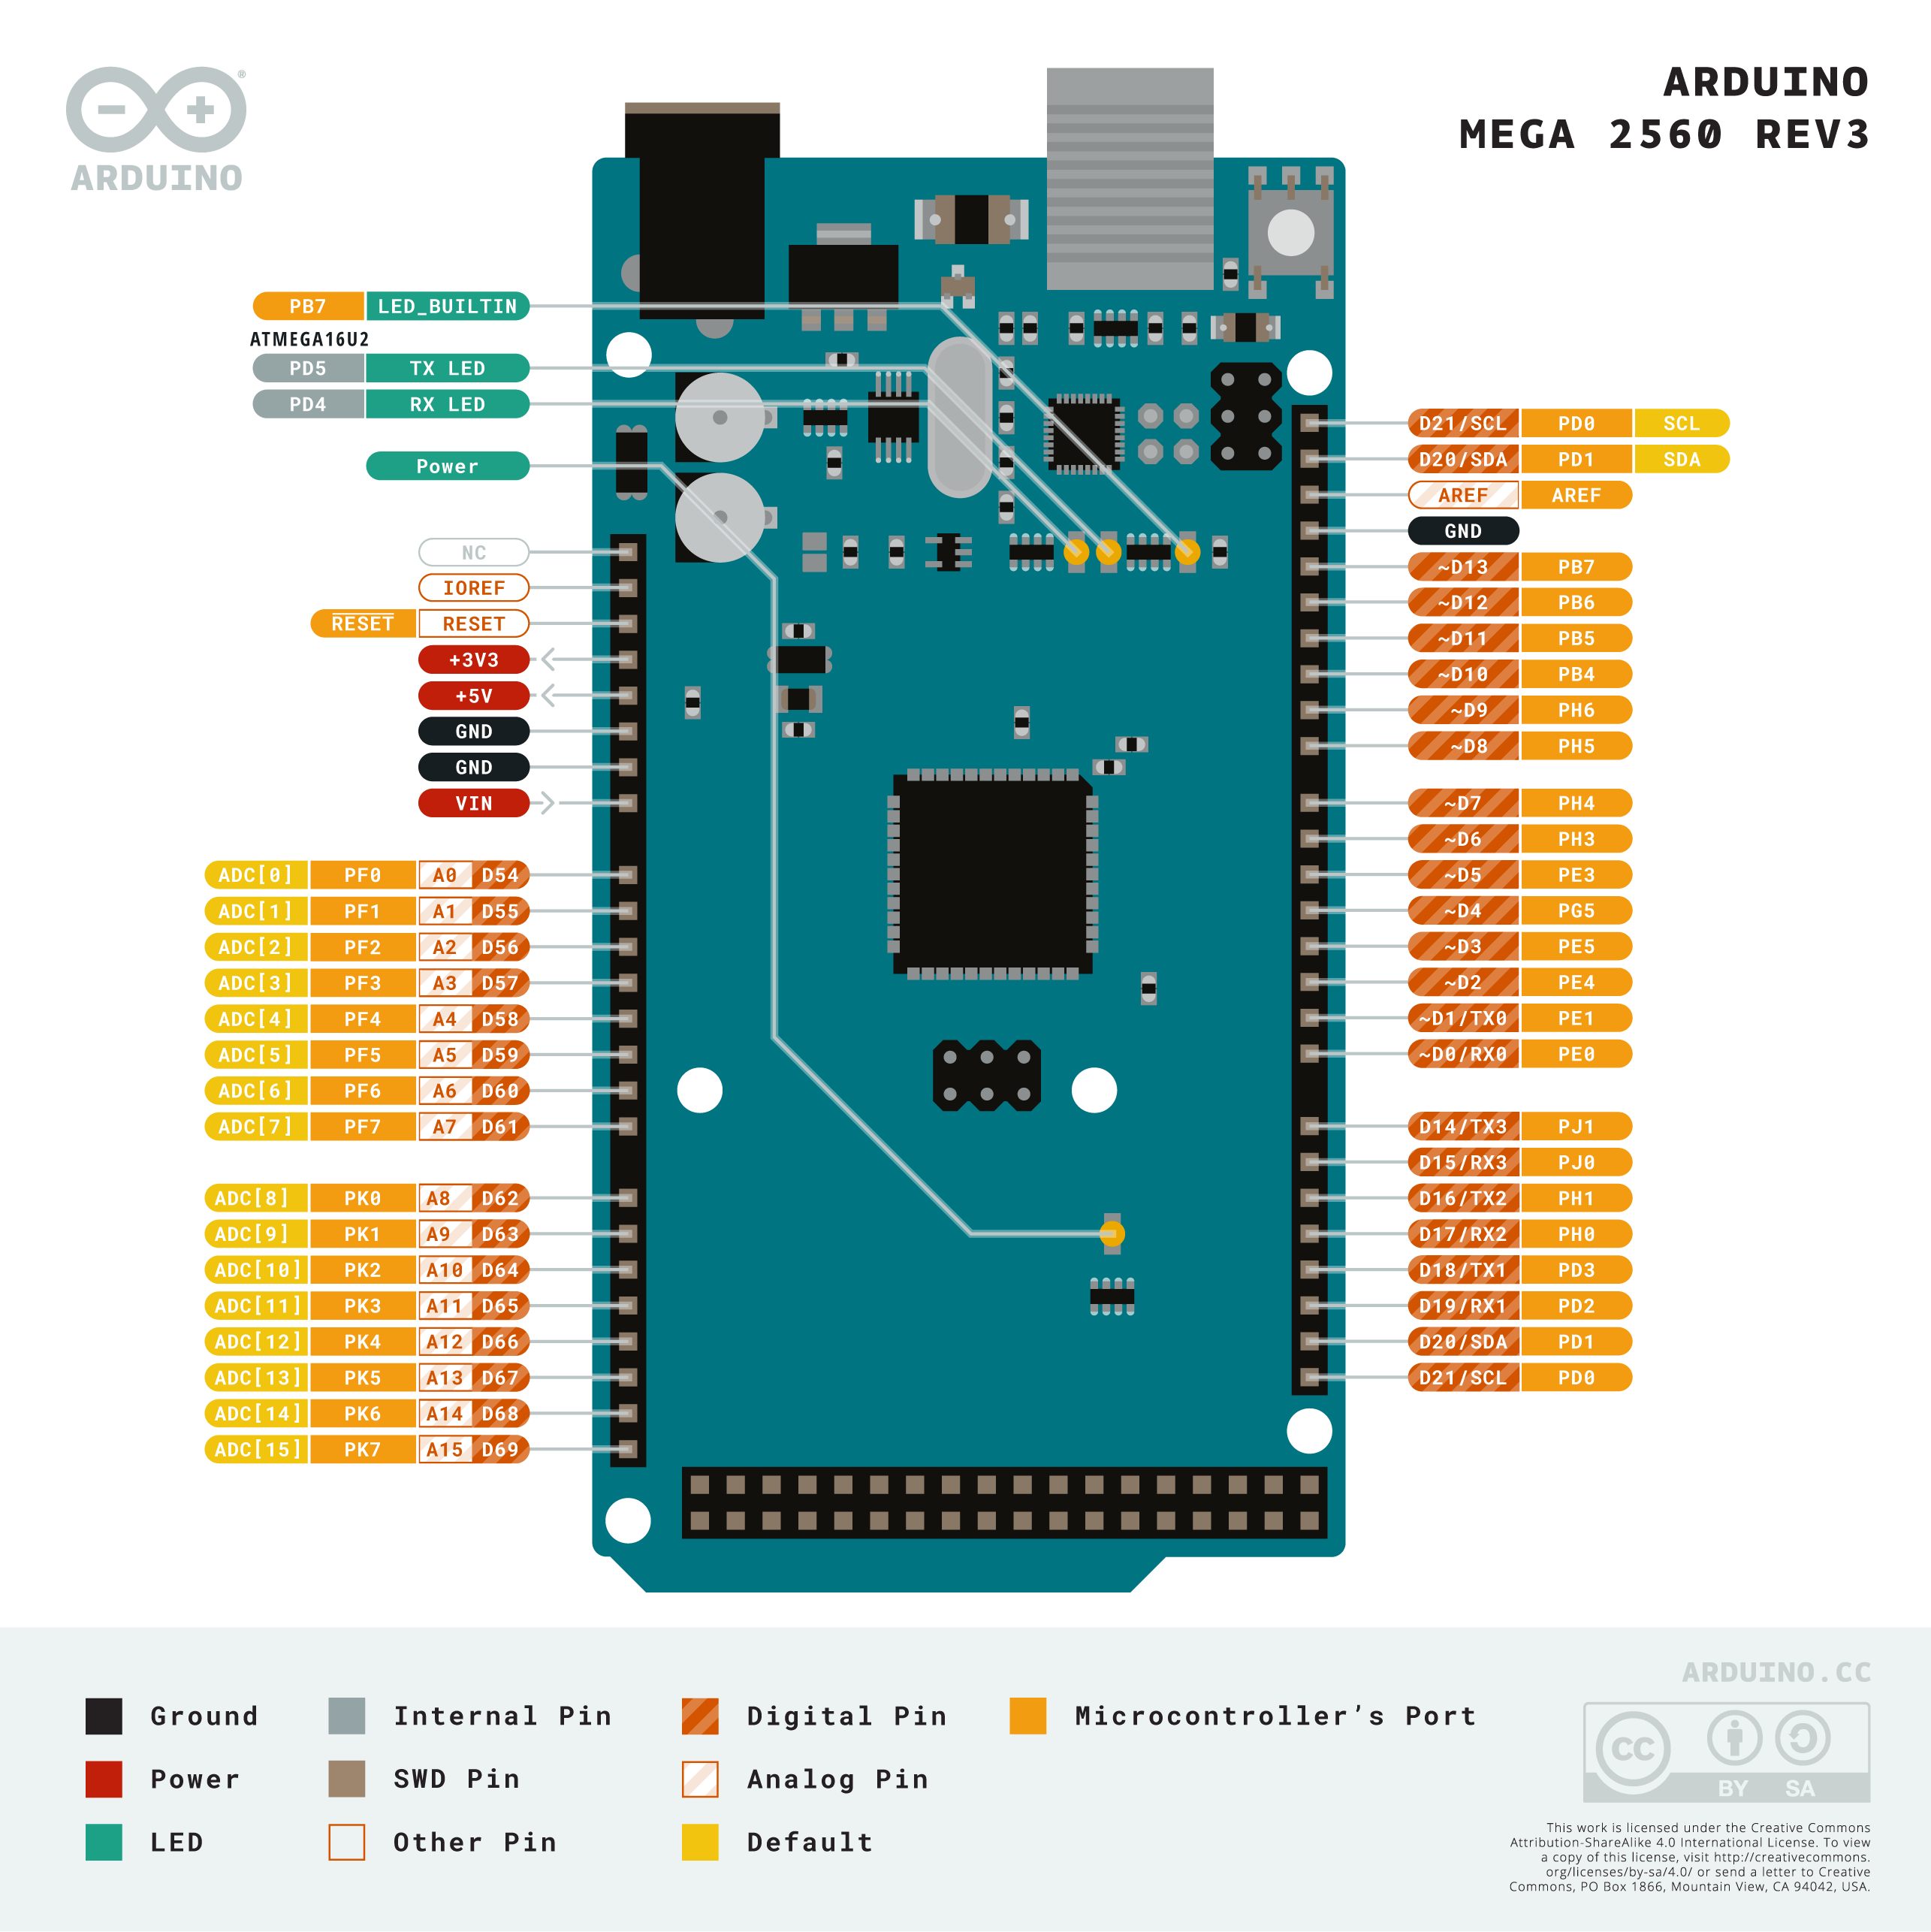
\includegraphics[scale=0.4]{figs/Pinout-Mega2560rev3-latest.png}
			\caption{
				شرح پین‌های \lr{Arduino Mega 2560 R3}
			}
			\label{fig:schema}
		\end{figure}
		
		\item {
			ماژول وای‌فای : \lr{ESP8266 ESP-01S}
			\footnote{
					این ماژول می‌تواند هم به عنوان یک نقطه دسترسی و هم به عنوان یک ایستگاه متصل به وای‌فای کار کند، بنابراین به راحتی داده‌ها را واکشی کرده و در اینترنت آپلود کند. همچنین می‌تواند با استفاده از \lr{API}، داده‌ها را از اینترنت واکشی کند و به هر اطلاعاتی که در اینترنت موجود است دسترسی داشته باشد. این ماژول فقط با ولتاژ 3.3 ولت کار می‌کند و هر ولتاژی بیش از 3.7 ولت باعث از بین رفتن ماژول می‌شود.
			}
		}
		
		\begin{figure}[H]
			\centering
			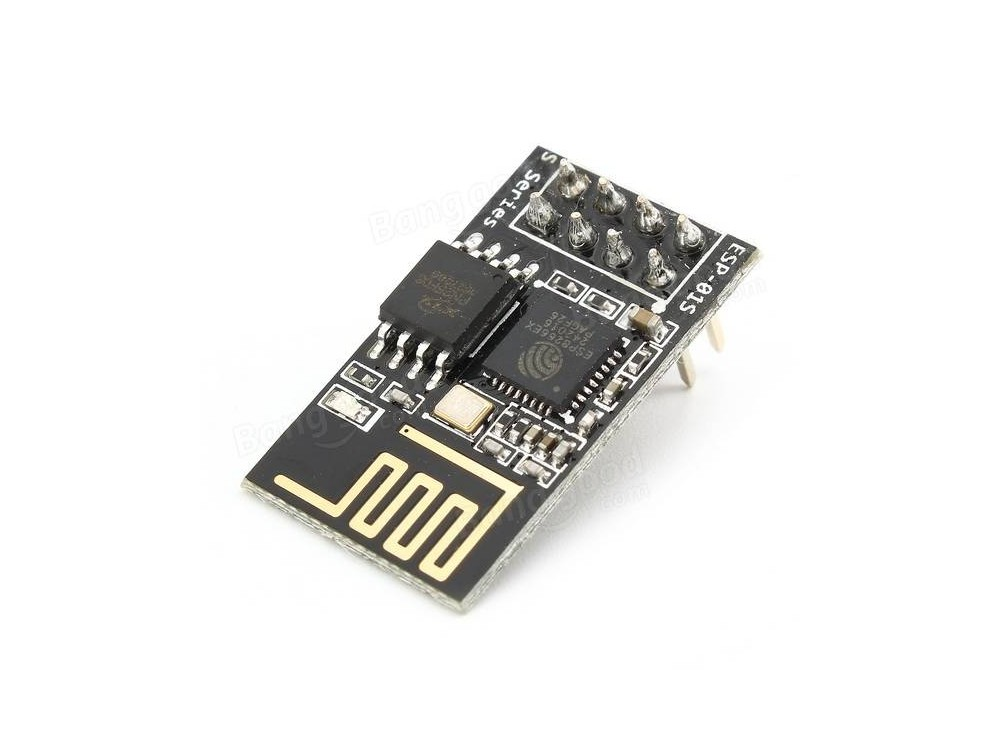
\includegraphics[scale=0.2]{figs/esp8266-esp-01s.jpeg}
			\caption{
				ماژول وای‌فای \lr{ESP8266 ESP-01S}
			}
			\label{fig:schema}
		\end{figure}
		
		\begin{figure}[H]
			\centering
			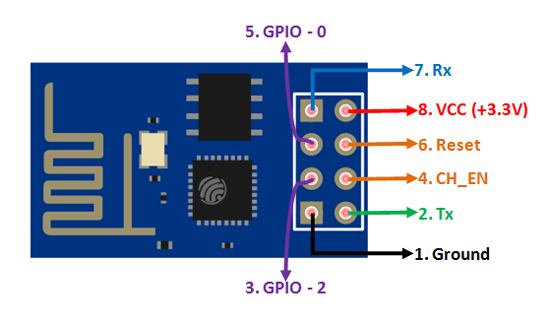
\includegraphics[scale=0.3]{figs/ESP8266-Pinout.png}
			\caption{
				شرح پین‌های \lr{ESP8266 ESP-01S}
			}
			\label{fig:schema}
		\end{figure}
		
		\begin{figure}[H]
			\centering
			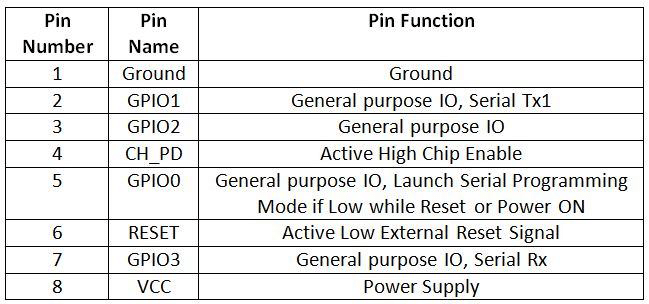
\includegraphics[scale=0.4]{figs/ESP-01-pin-configuration-The-RESET-and-VCC-pins-of-the-module-are-connected-to-the-33-V.png}
			\caption{
				تنظیمات پین‌های \lr{ESP8266 ESP-01S} (در اینجا پین \lr{GPIO1} همان \lr{TX} و \lr{GPIO3} همان \lr{TX} است. همچنین \lr{CH\_PD} معادل \lr{CH\_EN} در شرح پین است. )
			}
			\label{fig:schema}
		\end{figure}	
		
	\end{enumerate}
	
	
	\begin{itemize}
		\item 
		{تنظیم حساسیت سنسور نوری:} کاربر می‌تواند با انتخاب عددی میان ۱۰ الی ۱۵۰ (توسط \lr{slidebar})، میزان حساسیت سنسور نور را تنظیم کند (عدد کمتر معادل حساسیت کمتر است؛ یعنی میزان نور با تغییرات بیشتری نسبت به عددی بیشتر تغییر می‌کند).
		\item 
		{دکمه روشن و خاموش:} کاربر می‌تواند تمامی چراغ‌های لوستر (شاخه مورد نظر) را خاموش یا روشن کند.
		\item 
		{انتخاب شاخه:} کاربر می‌تواند انتخاب کند که متغیرهای تغییر داده شده، مربوط به کدام شاخه باشند (هر شاخه، مستقل از شاخه دیگر حالت‌های مختلف و دکمه‌های متفاوت دارد).
		\item 
		{حالت استاتیک یا داینامیک (\lr{Adaptive}):} کاربر می‌تواند با حالت استاتیک یک مقدار خاص را برای روشنایی انتخاب کرده و تمامی \lr{LED} های لوستر با آن مقدار تنظیم می‌شوند. در حالت داینامیک نیز مقدار روشنایی لوستر با سنسورهای تنظیم می‌شود.
		\item 
		{تنظیم حداکثر و حداقل میزان روشنایی:} کاربر می‌تواند با انتخاب عددی میان ۰ تا ۲۵۵(توسط \lr{slidebar})، حداقل و حداکثر میزان روشنایی یک شاخه را تعیین کند. بنابراین روشنایی یک شاخه، محدود به این دو عدد می‌شود و نمی‌تواند مقداری خارج از این بازه بگیرد.
		\item 
		{مودهای مختلف لوستر:} مودهای متفاوت که می‌توانند شامل لوستر را در حالت تنظیم داینامیک عادی یا رقص نور (همانند گزارش اول) تنظیم کنند (این حالت‌ها در قسمت‌های بعدی تکمیل می‌شوند). یکی از مودهای در نظر گرفته شده برای این قسمت حالت \lr{Inverted min to max} است که در آن نور دو شاخه به صورت معکوس با همدیگر کم و زیاد می‌شود.
		
	\end{itemize}
	همچنین برای ارتباط میان موبایل اپ و آردوییو به کمک ماژول \lr{ESP8266-07}، مدار را در مراحل زیر می‌بندیم (دقت کنید که هنگام آپلود کردن کد باید پین‌های \lr{RX} و \lr{TX} قطع شوند):
	\begin{enumerate}
		\item
		پین \lr{RX} در ماژول \lr{ESP} را به پین \lr{TX} آردویینو متصل می‌کنیم.
		\item
		پین \lr{TX} در ماژول \lr{ESP} را به پین \lr{RX} آردویینو متصل می‌کنیم.
		\item
		پین \lr{CH\_PD} یا \lr{Enable} در ماژول \lr{ESP} را به پین \lr{+3V} آردویینو متصل می‌کنیم.
		\item
		پین \lr{VCC} در ماژول \lr{ESP} را به پین \lr{+3V} آردویینو متصل می‌کنیم.
	\end{enumerate}
	
	در نهایت می‌توان با نصب کردن برنامه موبایل و اتصال آن به \lr{ESP} و آردویینو، تنظیمات موردنظر را انجام داد.
	\newpage
	در شکل زیر می‌توان شماتیک اپلیکیشن موبایل را دید.
	
	\begin{figure}[H]
		\centering
		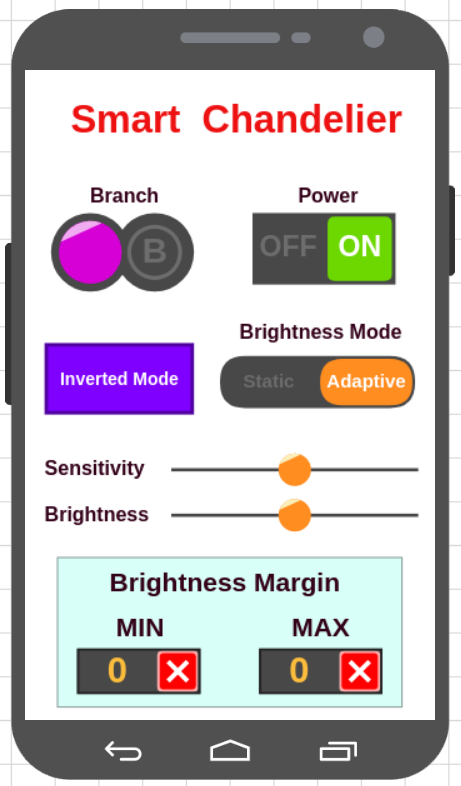
\includegraphics[scale=0.5]{figs/shcema-ma.png}
		\caption{
			شماتیک اپلیکیشن موبایل
		}
		\label{fig:schema}
	\end{figure}
	همین‌طور می‌توان کد آردویینو مربوط به این قسمت را مشاهده کرد. 
	
	%\begin{latin}
	%	\lstinputlisting[style={verilog-style}]{src/project.ino}
	%\end{latin}
	
\end{document}